% \\TODO: Eventually, instead of narrowing the focus to families of empirical data observed, everything available in marine and coastal ecosystems should be extracted from GloBI. This could be achieved rather easily.

% \\REVIEW: I am not convinced whether non-interactions are useful, as we are not even using them. Either we consider them in the algorithm to decrease probabilities of interactions are known to not happen, or we do not use them at all. I would tend to not use them since I am not convinced that non-interactions are valid data coming from food webs.

% \\REVIEW: I want to raise the question of the utility of non-interactions in the analyses. At this point, the algorithm is coded to ignore non-interactions in the similarity measurements. Maybe it would make sense to do the same in the interpretation of the results itself. Or a third vector to the similarity measurements could be added that considers non-interactions as a set of resources not consumed by consumers (which we have in the data). While this could make sense, more thought needs to be given to non-interactions stemming from empirical food webs and their actual value as observed data. If we think them valuable, then extra logical steps could be added to the algorithm to decrease probabilities of taxa being proposed as candidate resources by the KNN algorithm when they were observed to not interact in food webs.

% \\TODO: taxonomic similarity measure instead of tanimoto similarity

% \\IDEA: In an ideal world, another completely independant food web that was not used in the catalogue. Check stomach content data for St. Lawrence fish from IML, Denis Chabot. Claude Nozères is doing lab work on this, alternatively discuss with him first.

% \\REVIEW: Minimum threshold value to test and discuss. Completely arbitrary at this point.

% \\IDEA: Another interesting thought from this is the potential use of GloBI on its own to perform automated and quick analyses. If non-interactions are deemed unecessary or of dubious quality, focusing only on observed interactions could lead to the creation of a platform on which interactions in a given system could be easily predicted from GloBI alone, or almost. GloBI interactions data already holds taxonomic classification. It's quality is however unfortunately not uniform and care must be taken when it is used. In any case, if only interactions (1) are considered, then a third party platform could be built that uses the algorithm built in this paper, the GloBI data and a list of species for which we wish to predict the interactions.

\documentclass[letterpaper]{article}
\usepackage[utf8]{inputenc}
\usepackage{authblk}
\usepackage{hyperref}
\usepackage{graphicx}
\usepackage{makecell}
\usepackage{draftwatermark}
\SetWatermarkText{DRAFT}
\SetWatermarkScale{4}

\usepackage[usenames,dvipsnames,svgnames,table]{xcolor}

\definecolor{teal}{HTML}{008080}

\hypersetup {
  colorlinks = true, linkcolor = teal, citecolor = teal, urlcolor = teal,
  pdfauthor = {Beauchesne, David},
}

\renewcommand\Affilfont{\itshape\small}
\setcounter{section}{0}

\begin{document}

\title{
  \uppercase {Thinking outside the box - predicting biotic interactions in data-poor environments}
}
\uppercase{

\author[1*]{\textit{David Beauchesne}}
\author[2]{\textit{Philippe Desjardins-Proulx}}
\author[3]{\textit{Philippe Archambault}}
\author[2]{\textit{Dominique Gravel}}
}
\affil[*]{email: \href{mailto:david.beauchesne@uqar.ca}{david.beauchesne@uqar.ca}}
\affil[1]{Universit\'e du Qu\'ebec à Rimouski}
\affil[2]{Universit\'e de Sherbrooke}
\affil[3]{Université Laval}
\date{\today}
\maketitle

%ADD RUNNING TITLE HERE, MUST NOT EXCEEN 55 CHARACTERS AND SPACES

%UP TO 8 KEYWORDS
% \keywords{predicting biotic interactions, machine learning, food webs, estuary and gulf of St.Lawrence}

\newpage

% ---------------------------------
% ---------------------------------
%           ABSTRACT
% ---------------------------------
% ---------------------------------
\section{Abstract} % about 200 words
% \\TODO: verify 94 food webs

Large networks of ecological interactions, such as food webs, are complex to characterize, be it empirically or theoretically. The former requires exhaustive observations, while the latter generally requires ample data to be validated. We therefore wondered whether readily available data, namely empirically described interactions in a variety of ecosystems and taxonomy, could be combined to predict species interactions in data deficient ecosystems. To test this, we built a biotic interactions catalogue from a collection of \textit{94} empirical food webs, detailed predator-prey interaction databases and interactions from the Global Biotic Interactions (GloBI) database. We used an unsupervised machine learning method to predict interactions between any given set of taxa, given pairwise taxonomic proximity and known consumer and resource sets found in the interaction catalogue. Initial results suggest that pairwise interactions can be predicted with high accuracy. Although results are seemingly dependent on the comprehensiveness of the catalogue rather than the taxonomic similarity between taxa, taxonomy was found to complement well the catalogue and to allow the algorithm to perform well when the amount of information available through the catalogue decreased. Given it’s high accuracy, this methodology could democratize the use of food webs and network level descriptors in remote location where empirical data is hard to gather. Network characteristics could then be efficiently evaluated and correlated to levels of environmental stressors in order to improve vulnerability assessments of ecosystems to global changes, opening promising avenues for further research and for management initiatives.

% ---------------------------------
% ---------------------------------
%           INTRODUCTION
% ---------------------------------
% ---------------------------------
\section{Introduction}
% \\REVIEW: verify source, Eklof et al 2012 for this citation, not 100% certain that's where it comes from

Large networks of ecological interactions, such as food webs, are complex to characterize, be it empirically or theoretically. The former requires exhaustive observations, while the latter generally requires ample data to be validated. For this reason, studies focusing on communities of interacting species remain understudied even though we acknowledge the importance of considering the reticulated nature of complex networks (ref). When time is of the essence, the long term studies required quickly become impractical and the use of network level approaches relegated to the sideline (ref).

Alternatively, a currently evolving approach is to predict interactions using proxies such as functional traits, phylogenies and spatial distributions (e.g. Gravel et al., 2013; Morales-Castilla et al., 2015). For example, multiple traits can play a significant role in community dynamics and influence the presence and intensity of biotic interactions, like the influence of body size on predator-prey interactions, a literal take on \textit{big fish eats small fish} (Cohen et al., 2003; Brose et al., 2006; Gravel et al. 2013). However, the time required to gather the necessary data to apply those methods may still be restrictive, or the data be unavailable altogether, so much so that other methods have been developed to fill the gaps in knowledge (e.g. Schrodt et al. 2016).

We therefore wondered whether more readily available data could be used to infer interactions in data deficient ecosystems. There is an increasing amount of data available describing worldwide species interactions, some freely available through the Global Biotic Interactions (GloBI) database (Poelen et al. 2014). Another readily available piece of information on species is their taxonomy, through initiatives like the World Register of Marine Species (WoRMS; Bailly et al. 2016). More than simple nomenclature, evolutionary processes are thought to influence consumer-resource relationships so that taxonomically related species would be more likely to share similar types of both consumers and resources (Eklof et al. 2012; Morales-Castilla et al. 2015). Based on that assumption, taxonomy might be useful in predicting interactions for species lacking detailed information, but which have a taxonomically related species for which such information is available. The objective of this work is thus to combine empirical biotic interactions originating from a variety of ecosystems with taxonomic relatedness to predict interactions in data deficient ecosystems.

% ---------------------------------
% ---------------------------------
%             METHODS
% ---------------------------------
% ---------------------------------
\section{Methods}
The objective of the methodology presented is to predict the interactions between all taxa within an arbitrary set \textit{S1} using a set of taxa \textit{S0} with empirically described interactions from which we can extract sets of consumers and resources and their taxonomy. We couple the use of empirical data with an unsupervised machine learning method to achieve this.

 \subsection{Biotic interaction catalogue}
   % \\REVIEW: Verify 'scientific nomenclature'
   % \\TODO: Appendix 1 Description of food web used. The majority come from GlobalWeb
   % \\TODO: Add reference GlobalWeb database (http://globalwebdb.com)
   % \\TODO: Verify references to add
   % \\TODO: Add GloBI; http://www.globalbioticinteractions.org
   % \\REVIEW: Verify number of taxa and number per taxa for first data compilation step

We built a biotic interaction catalogue to serve as a set of taxa \textit{S0} with empirically described interactions. The empirical data used to construct the interaction catalogue was gathered in two successive steps. The first consisted of gathering data from a collection of 94 empirical food webs in marine and coastal ecosystems from which we extracted pairwise taxa interactions (Brose et al. 2005; Kortsch et al. 2015; GlobalWeb database). We also used a detailed predator-prey interaction database describing trophic relationships between \textit{XX} predators and their prey (Barnes et al. 2008). From these datasets, only interactions between taxa at the taxonomic scale of the family or higher were selected for inclusion in the catalogue.

As empirical food webs are vastly dominated by non-interactions, these datasets yielded a highly skewed distribution of interactions vs non-interactions. To counterbalance this, the second step of data compilation consisted of extracting observed interactions from the Global Biotic Interaction (GloBI) database (ref), which describes binary interactions for a wide range of taxa worldwide. We extracted all interactions available on GloBI for species belonging to the families of taxa identified through step 1. Interactions were extracted using the rGloBI package in R (ref). As for step 1, only interactions between taxa at the taxonomic scale of the family or higher were retained

The nomenclature used between datasets and food webs varied substantially. Taxa names thus had to be verified, modified according to the scientific nomenclature and validated. This process was performed using the Taxize package in R (ref) and manually verified for errors. The same package was used to extract the taxonomy of all taxa for which interactions were obtained in previous steps. The complete R code and data used for the catalogue is available at \href{https://github.com/david-beauchesne/Interaction_catalog}{https://github.com/david-beauchesne/Interaction\_catalog}.

  \subsection{Unsupervised machine learning}
We use the \textit{K}-nearest neighbor (KNN) algorithm (\textbf{ref}) to predict pairwise interactions for a set of taxa \textit{S}. The KNN algorithm predicts missing entries or proposes additional entries by a majority vote based on the \textit{K} nearest (\textit{i.e.} most similar) entries. In this case, taxa are described by a set of resources when considered as a consumer, a set of consumers when considered as a resource and their taxonomy (\textit{i.e.} kingdom, phylum, class, order, family, genus, species). Similarity between taxa was evaluated using the Tanimoto similarity measure (\textbf{ref}), which compares two vectors with \textit{i} elements based on the number of elements they share and contain:

\begin{equation}
  tanimoto(\mathbf{x}, \mathbf{y}) = \frac{\sum_i x_i \land y_i}{\sum_i x_i \lor y_i},
\end{equation}

where $\land$ is bitwise \emph{and}, while $\lor$ is the bitwise \emph{or} operators. Adding a weighing scheme, we can measure the similarity using two different sets of vectors with \textit{i} and \textit{j} elements, respectively.

\begin{equation}
  tanimoto_t(\mathbf{x}, \mathbf{y}, w_t) = w_ttanimoto(\mathbf{x_i}, \mathbf{y_i}) + (1 - w_t)tanimoto(\mathbf{x_j}, \mathbf{y_j}),
\end{equation}

where $w_t$ is the weight given to vector \textit{i}, $\mathbf{x_i}$, $\mathbf{y_i}$ are the resource or consumer sets of the two taxa and $\mathbf{x_j}$ and $\mathbf{y_j}$ are the vectors for the taxonomy of two taxa. When $w_t$ = 0 only resource or consumer sets are used to compute similarity, while $w_t$ = 1 solely uses taxonomy.

  \subsection{Predicting interactions, Biotic predictor algorithm, Two-way Tanimoto algorithm, Feng shui name algorithm, Find a name for the algorithm}
  % \\REVIEW: In the algorithm paragraph I do not discuss the following parameters, but should I? Right now they are in Figure \ref{fig:decision_diag} though.
  % \\REVIEW: Minimum weight: minimum weight for candidate taxa to make it to predictions
  % \\REVIEW: Minimum threshold: arbitrary value set to 0.3 (no scientific basis) for similarities. If under, KNN taxa are not retained as potential candidates and their weight is not added to the candidate taxa list. It seems trivial, technically if their similarity is so low it shouldn't interfere with results? It does in cases like the atlantic cod, which has over 600 listed resources. In that case, the iterative process goes through them all and a species with a similarity = 0.05 could end up adding a total of 30 to it's weight in the candidate list. We had two choice to deal with this issue. Either we set a variable MW that varies as a function of the number of candidate resources, or we set another minimum threshold for resource to make it into the candidate list, effectively resulting in two arbitrarily chosen values for the predictions.
  % \\REVIEW: Cannibalism not allowed in this iteration of the algorithm, but it is present in empirical webs. Should be added at some point.
  % \\IDEA: Present an example that goes through the algorithm logical steps

The XXX algorithm is built on a series of logical steps that ultimately predicts a candidate resources list $C_R$ for each taxon in \textit{S1} (Figure \ref{fig:decision_diag}). For all consumer taxa $T_C$ in \textit{S1}, the algorithm first verify whether it has empirical resources $T_R$ listed in the catalogue. When it does, if $T_R$ are also in \textit{S1}, they are added as predicted resources for $T_C$. This corresponds to what we refer to as the catalogue contribution to resource predictions. Two taxa in \textit{S1} that are known to interact through the catalogue are automatically assumed to interact in \textit{S1}.

Otherwise, the algorithm passes to what we refer to as the predictive contribution to resource predictions, with candidate resources for $T_C$ identified with the KNN algorithm. If $T_R$ are also in \textit{S1}, K most similar resource $T_{R'}$ are identified in \textit{S1} to add to $C_R$. Then for all $T_C$ in \textit{S1}, the algorithm identifies K most similar consumer $T_{C'}$ in \textit{S0} and extracts their resource sets. As before, if those resources are found in \textit{S1} they are added to $C_R$, otherwise K most similar resources $T_{R'}$ are identified in \textit{S1} to add to $C_R$. A simple working example is presented at Figure \ref{fig:example}. Other parameters are used in the algorithm, but not presented here for the sake of message clarity. A more comprehensive mathematical description of the algorithm and the parameters used is however available through Figure \ref{fig:decision_diag} and the complete R code and data used for the algorithm is available at \href{https://github.com/david-beauchesne/Predict_interactions}{https://github.com/david-beauchesne/Predict\_interactions}.


\subsection{Algorithm prediction accuracy}
We used the most extensive and taxonomically detailed datasets included in the catalogue (\textbf{ref}) to assess the prediction accuracy of the algorithm. Testing accuracy of a particular dataset was done by first removing from the catalogue all pairwise interacting originating from that dataset. Accuracy was evaluated using three different statistics:

\begin{enumerate}
 \item $Score_y$ is the fraction of interactions correctly predicted:
     \begin{equation}
         Score_y = \frac{a}{a + c}
     \end{equation}

 \item $Score_{\neg y}$ is the fraction of non-interactions correctly predicted:
     \begin{equation}
       Score_{\neg y}  = \frac{d}{b + d}
     \end{equation}

 \item TSS, The True Skilled Statistics (TSS) evaluated prediction success by considering both true and false predictions, returning a value ranging from 1 (prefect predictions) to -1 (inverted predictions; \textbf{ref}): %Allouche, Tsoar et Kadmon 2006; Gravel et al. 2013
     \begin{equation}
       TSS = \frac{(ad - bc)}{(a + c)(b + d)}
     \end{equation}
\end{enumerate}

where a is the number of links predicted (1) and observed (1), b is the number predicted (1) but not observed (0), c is the number predicted absent (0) but observed (1) and d is the number of predicted absent (0) and observed absent (0). These three statistics give a different perspective on prediction accuracy, focusing in turn on true interactions and non-interactions, and on both true and false predictions.

We evaluated the three statistics for the complete algorithm and for the catalogue and the predictions individually to evaluate their respective contribution to the algorithm predictive accuracy. Multiple $w_t$ values were also tested to evaluate whether taxa similarity measured as a function of resource/consumer sets or taxonomy contributed more significantly towards increased predictive accuracy. The same was done with multiple $K$ values.

Finally, we evaluated the influence of the comprehensiveness of the catalogue on prediction accuracy. We selected the arctic food web from Kortsch et al. (2015). This food web was selected as it is highly detailed taxonomically and because empirical data remains available for most of its taxa after its exclusion from the catalogue. We iteratively and randomly ($n$ = 50) removed a percentage of empirical data describing the food web taxa from the catalogue before generating new predictions with the algorithm. We also tested $w_t$ values of 0.5 and 1 to evaluate whether taxonomic similarity could support predictive accuracy in cases when empirical data for species in \textit{S1} in the catalogue is unavailable.

\subsection{Southern Gulf of Saint Lawrence}
    As an example, we used the XXX algorithm to predict interactions in the Southern Gulf of Saint Lawrence (SGSL) in eastern Canada. The empirical data and taxa list come from Savenkoff et al. (2004). They present a list of 29 functional groups for a total of 80 taxa. As their analysis was performed on the functional groups rather than the taxa themselves, we used the algorithm to predict interactions between all 80 taxa, which we aggregated back to their original functional groups to compare with interactions presented in Savenkoff et al. (2004).

% ---------------------------------
% ---------------------------------
%            RESULTS
% ---------------------------------
% ---------------------------------
% \\TODO: Not MW, MT and accuracy score. The goal of the paper is to present the methodology and it just takes away from my main message. Accuracy score is taken out mainly because as non-interations vastly outnumber interactions, that graph essentially gives the same information as the score -y one. So now we would have three statistics instead of 4. Makes more sense I believe.
% \\TODO: include name of datasets used in figure captions

\section{Results}
    \subsection{Biotic interaction catalogue}
The data compilation process allowed us to build an interaction catalogue composed of 276708 pairwise interactions (interactions = 72110; non-interactions = 204598). A total of 9712 taxa (Superfamily = 15; Family = 591; Subfamily = 29; Tribe = 8; Genus = 1972; Species = 7097) are included in the catalogue, 4159 of which have data as consumers and 4375 as resources.

    \subsection{Algorithm predictive accuracy}
The overall predictive accuracy of the algorithm ranges between 80\% to almost 100\% in certain cases (Figure \ref{fig:multi_param}), except for one food web (\textit{i.e.} \textbf{ref}). Both interactions and non-interactions are well predicted by the algorithm. TSS scores are lower than $Score_y$ and $Score_{\neg y}$ due to misclassified interactions and non-interactions. This can also be observed through the effect of varying $K$ values, which increases the number of potential candidate resources for each taxa in the predictive portion of the algorithm. Prediction accuracy increases for interactions, while it decreases for non-interactions, as $K$ values increase.

Similarity being predominantly measured with resource/consumer sets ($w_t$ closer to 0) yielded better predictions than when measured with taxonomy ($w_t$ closer to 1; Figure \ref{fig:multi_param}). Resource/consumer sets therefore appears to serve as a better predictor of similarity between taxa for interactions predictions. It is nonetheless interesting to note that although the predictive contribution of the algorithm decreases as $w_t$ increases, an increased mean and decreased variability values for the TSS and $Score_y$ statistics is also observed (Figure \ref{fig:multi_param})). This suggests that while using taxonomy for similarity measurements yields lower predictive accuracy, it may also complement the catalogue contribution by predicting interactions not captured through empirical data, effectively increasing the predictive accuracy of the complete algorithm.

The partitioning of the catalogue and predictive portions of the algorithm shows that it is dependent on the comprehensiveness of the catalogue for high prediction accuracy (Figures \ref{fig:multi_param}, \ref{fig:catalog_pred}). As the amount of empirical data available in the catalogue decreases so does the overall accuracy of the algorithm (Figures \ref{fig:catalog_pred}). The predictive contribution of the algorithm however slows down the decrease in the prediction efficiency of the algorithm. Prediction accuracy still remains around 75\% with only 40\% of \textit{S1} taxa found in the catalogue (Figures \ref{fig:catalog_pred}). Furthermore, the use of taxonomy for similarity measurements is more efficient as empirical data becomes scarcer and no different than resource/consumer sets for the complete algorithm when ample data is available (Figures \ref{fig:catalog_pred}).

    \subsection{Southern Gulf of Saint Lawrence}
In total, there were empirical data available through the catalogue for 53 out of 80 SGSL taxa. The XXX algorithm correctly predicted approximately 75\% of interactions ($a$) and non-interactions ($d$) extracted from Savenkoff et al. (2004). It however predicted an additional 113 interactions ($c$) that were not noted in Savenkoff et al. (2004) and failed to predict 44 observed interactions that were ($c$).


%     a           b           c           d         TSS     ScoreY1     ScoreY0         FSS
% 126.0000000 113.0000000  44.0000000 342.0000000   0.4928248   0.7411765   0.7516484   0.7488000

% ---------------------------------
% ---------------------------------
%           DISCUSSION
% ---------------------------------
% ---------------------------------
\section{Discussion}
We show that out of the box interaction inference for a set of taxa with incomplete or unavailable preexisting information can be achieved with high accuracy using a combination of empirical data describing biotic interactions and taxonomic relatedness. Although the efficiency of the algorithm is dependent on the comprehensiveness of the interactions catalogue, taxonomic proximity acts as a complement to increase the number of observed interactions correctly predicted. Taxonomic proximity also supports the efficiency of the algorithm when catalogue comprehensiveness decreases. Overall, we believe that the methods performs well and offers promising avenues for further research and management initiatives.

\subsection{Algorithm accuracy}




\subsection{Interactions classification}
The $Score_{y}$ and $Score_{\neg y}$ are inversely proportional. This means that non-interactions are misclassified as interactions in the process of increasing $Score_y$, consequently decreasing $Score_{\neg y}$. This could either stem from the algorithm poorly predicting non-interactions or from the empirical data itself. Accuracy evaluation assumes that non-interactions from empirical food web are observed data, yet it is usually not the case. Most empirical webs have a strong focus attributed to higher order consumer species and very little attention given to other taxa (\textbf{ref}). Furthermore, the methodologies used to obtain consumer-resource data usually relies in gut content analyses, which is efficient at observing interactions, but not so for absence of interactions (\textbf{ref}). Misclassified interactions could thus be real, albeit unobserved through empirical data available. It should however be noted that impossible interactions are still predicted by the algorithm, like atlantic cod (\textit{Gadus morhua}) and large demersal feeders such as the atlantic halibut (\textit{Hippoglossus hippoglossus}) consuming whales and birds.

\subsection{Southern Gulf of Saint Lawrence}



Ok, so the fact that it is not that well predicted, that we predict more

We can break down functional groups for a more thorough understanding of individual components of the network rather than the aggregated version.

With 80 species, it isn't such a big deal, but the whole Saint Lawrence comprises over 1300 species. Grouping species in functional groups makes more sense. Forming functional groups based on their interactions with other species, i.e. describing analytically identified groups, could provide a new way of aggregating species together and at the same time evaluate whether original functional groupings made sense.

Something else that could be done is to reevaluate




\subsection{Usefulness of taxonomic relatedness}
 While we found that taxonomy could be useful as a complement to predictions made using empirical data, the accuracy of predictions made using the KNN algorithm are quite low. Other uses of this machine learning approach have been known to achieve much higher prediction rates (\textit{e.g.} \textbf{refs}), which leaves us to believe that taxonomy is not the optimal proxy for predicting interactions. While evolutionary history plays a significant role in influencing consumer-resource trait matching and food web structure (\textbf{ref}), phylogenetic constraints does not account efficiently for certain traits such as body size (Eklöf and Stouffer 2015). Including traits like body size and metabolism as an additional component of this algorithm could thus help increasing overall prediction accuracy, especially in cases where the catalogue lacks data on taxa for which interactions have to be predicted. Although promising, such an approach would undermine the premise under which this method was built and which constitutes its main strength, predicting interactions in data deficient environments using readily available data.





\subsection{Perspectives}
Given the efficiency and simplicity of the XXX algorithm,

The simplicity of the XXX algorithm could prove useful for a variety of reasons



Given it’s high accuracy, this methodology could democratize the use of food webs and network level descriptors in remote location where empirical data is hard to gather. Network characteristics could then be efficiently evaluated and correlated to levels of environmental stressors in order to improve vulnerability assessments of ecosystems to global changes, opening promising avenues for further research and for management initiatives.



Democratizing the use of network level predictors
Management
Applied research in theoretical ecology
Adding interaction strength to predictions












\section{Acknowledgements}
We thank the Fond de Recherche Québécois Nature et Technologie (FRQNT) and the Natural Science and Engineering Council of Canada (CRSNG) for financial support. This project is also supported by Québec Océan, the Quebec Centre for Biodiversity Science (QCBS), and the Notre Golfe and CHONeII networks. We also wish to thank K. Cazelles for constructive comments and suggestions.

\newpage
\subsection{Box 1}
The XXX algorithm follows a series of logical steps to predict resources for all taxa in an arbitrary set of taxa \textit{S1} using a set of taxa \textit{S0} with empirically described interactions from which we can extract sets of consumers and resources and their taxonomy. In this example, we are predicting interactions for a fictitious \textit{S1}
 = $\{T_1, T_9, T_{10},T_{11}, T_{12}\}$ using \textit{S0} with information on 12 taxa. This catalogue holds information on consumer or resource for 10 taxa and the taxonomy for all 12 taxa in the list.

    \begin{table}[h!]
      \centering
      \begin{tabular}{cccc}
        \hline
        \textit{S0} taxa ID & taxonomy &          resource &             consumer        \\
        \hline
        \hline
        $T_1$ &         $\{a, b, c\}$ &     $\{T_2, T_3, T_{12}\}$ &    $\{T_4\}$         \\
        $T_2$ &         $\{e, f, g\}$ &      &                          $\{T_1, T_5\}$    \\
        $T_3$ &         $\{i, j, k\}$ &      &                          $\{T_5\}$         \\
        $T_4$ &         $\{m, n, o\}$ &     $\{T_1, T_5\}$ &                              \\
        $T_5$ &         $\{a, b, d\}$ &     $\{T_8, T_9\}$ &            $\{T_4\}$         \\
        $T_6$ &         $\{i, q, r\}$ &     $\{T_2, T_8\}$ &            $\{T_4\}$         \\
        $T_7$ &         $\{e, f, h\}$ &      &                          $\{T_1, T_6\}$    \\
        $T_8$ &         $\{s, t, u\}$ &      &                          $\{T_5, T_6\}$    \\
        $T_9$ &         $\{s, t, v\}$ &      &                          $\{T_5\}$         \\
        $T_{10}$ &      $\{i, j, l\}$ &      &                                            \\
        $T_{11}$ &      $\{m, n, p\}$ &      &                                            \\
        $T_{12}$ &      $\{q, r, s\}$ &      &                          $\{T_1\}$         \\
        \hline
      \end{tabular}
    \end{table}

Similarity between all pairs of taxa in \textit{S0} is measured for consumer, resource and taxonomic proximity using equation 1. The upper triangular matrix represents similarity measured with taxa sets of resources/consumers, while the lower triangular represents taxonomic similarities. For consumer/resource set similarities, values of 0 mean that similarity equals 0 for both similarity measurements.
\bigskip

    \centerline{$tanimoto(T_Cx, T_Cy)$ / $tanimoto(T_Rx, T_Ry)$ }

    \begin{table}[h!]
      \centering
      \small
      \begin{tabular}{c|ccccccccccccc}
        & $T_1$ & $T_2$ & $T_3$ & $T_4$ & $T_5$ & $T_6$ & $T_7$ & $T_8$ & $T_9$ & $T_{10}$ & $T_{11}$ & $T_{12}$ \\
        \hline
        $T_1$       & -     & 0     & 0         & 0     & 0/1   & 0.3/1     & 0         & 0         & 0         & 0     & 0     & 0         \\
        $T_2$       & 0     & -     & 0/0.5     & 0     & 0     & 0         & 0/0.3     & 0/0.3     & 0/0.5     & 0     & 0     & 0/0.5     \\
        $T_3$       & 0     & 0     & -         & 0     & 0     & 0         & 0         & 0/0.5     & 0/1       & 0     & 0     & 0         \\
        $T_4$       & 0     & 0     & 0         & -     & 0     & 0         & 0         & 0         & 0         & 0     & 0     & 0         \\
        $T_5$       & 0.5   & 0     & 0         & 0     & -     & 0.3/1     & 0         & 0         & 0         & 0     & 0     & 0         \\
        $T_6$       & 0     & 0     & 0.2       & 0     & 0     & -         & 0         & 0         & 0         & 0     & 0     & 0         \\
        $T_7$       & 0     & 0.5   & 0         & 0     & 0     & 0         & -         & 0/0.3     & 0         & 0     & 0     & 0/0.5     \\
        $T_8$       & 0     & 0     & 0         & 0     & 0     & 0         & 0         & -         & 0         & 0     & 0     & 0         \\
        $T_9$       & 0     & 0     & 0         & 0     & 0     & 0         & 0         & 0.5       & -         & 0     & 0     & 0         \\
        $T_{10}$    & 0     & 0     & 0.5       & 0     & 0     & 0.2       & 0         & 0         & 0         & -     & 0     & 0         \\
        $T_{11}$    & 0     & 0     & 0         & 0.5   & 0     & 0         & 0         & 0         & 0         & 0     & -     & 0         \\
        $T_{12}$    & 0     & 0     & 0         & 0     & 0     & 0.5       & 0         & 0.2       & 0.2       & 0     & 0     & -         \\
      \end{tabular}
    \end{table}

    \centerline{$tanimoto(T_Tx, T_Ty)$}
\bigskip

From these, the algorithm goes through logical steps to identify a candidate resource list $C_R$ for each taxon in \textit{S1} using either empirical data directly or $K$ most similar taxa with equation 2. Going through the process for $T_1$, using $K$ = 1 and $w_t$ = 1:
\bigskip

\begin{table}[h!]
  \centering
  \begin{tabular}{l}
      Steps \\
      \hline
      \textbf{1)} $I(T_1,T_R)$ in \textit{S1}? \\
      $T_2$ = no $\rightarrow$ $t(T_2, T_{R'}, w_t)$ = NA   \\
      $T_3$ = no $\rightarrow$ $t(T_2, T_{R'}, w_t)$ = $T_{10}$ = 0.5 \\
      $T_{12}$ = yes    \\  \\
      \textbf{2)} $t(T_1, T_{C'}, w_t)$ = $T_5$ = 0.5            \\
      I($T_5$,$T_R$) in \textit{S1}? \\
      $T_8$ = no $\rightarrow$ $t(T_8, T_{R'}, w_t)$ = $T_9$ = 0.5  \\
      $T_9$ = yes   \\
  \end{tabular}
  \quad
  \begin{tabular}{c|c}
      \\  \\  \\  \\  \\  \\  \\  \\  \\
  \end{tabular}
  \quad
  \begin{tabular}{cc}
      Catalogue   & Predictions \\
      \hline \\
      $\{\}$    & $\{\}$            \\
      $\{\}$    & $\{T_{10}\}$      \\
      $\{T_{12}\}$    & $\{T_{10}\}$      \\  \\  \\ \\
      $\{T_{12}\}$    & $\{T_9, T_{10}\}$      \\
      $\{T_9, T_{12}\}$    & $\{T_9, T_{10}\}$      \\
  \end{tabular}
\end{table}
\bigskip

The logical steps allow us to predict a set of resources for $T_1$ = {$T_9$, $T_{10}$, $T_{12}$}. Doing it for all taxa in \textit{S1} with $w_t$ = 0 and 1 predicts the following networks:
\bigskip

\centerline{\textbf{$w_t$ = 0 \quad \quad \quad \quad \quad $w_t$ = 1} \quad}
    \begin{figure}[h!]
    \centering\includegraphics[height = 6cm]{example.pdf}
    \end{figure}
% Example finish

\newpage
\subsection{Figures}
    \begin{figure}[h]
      \centering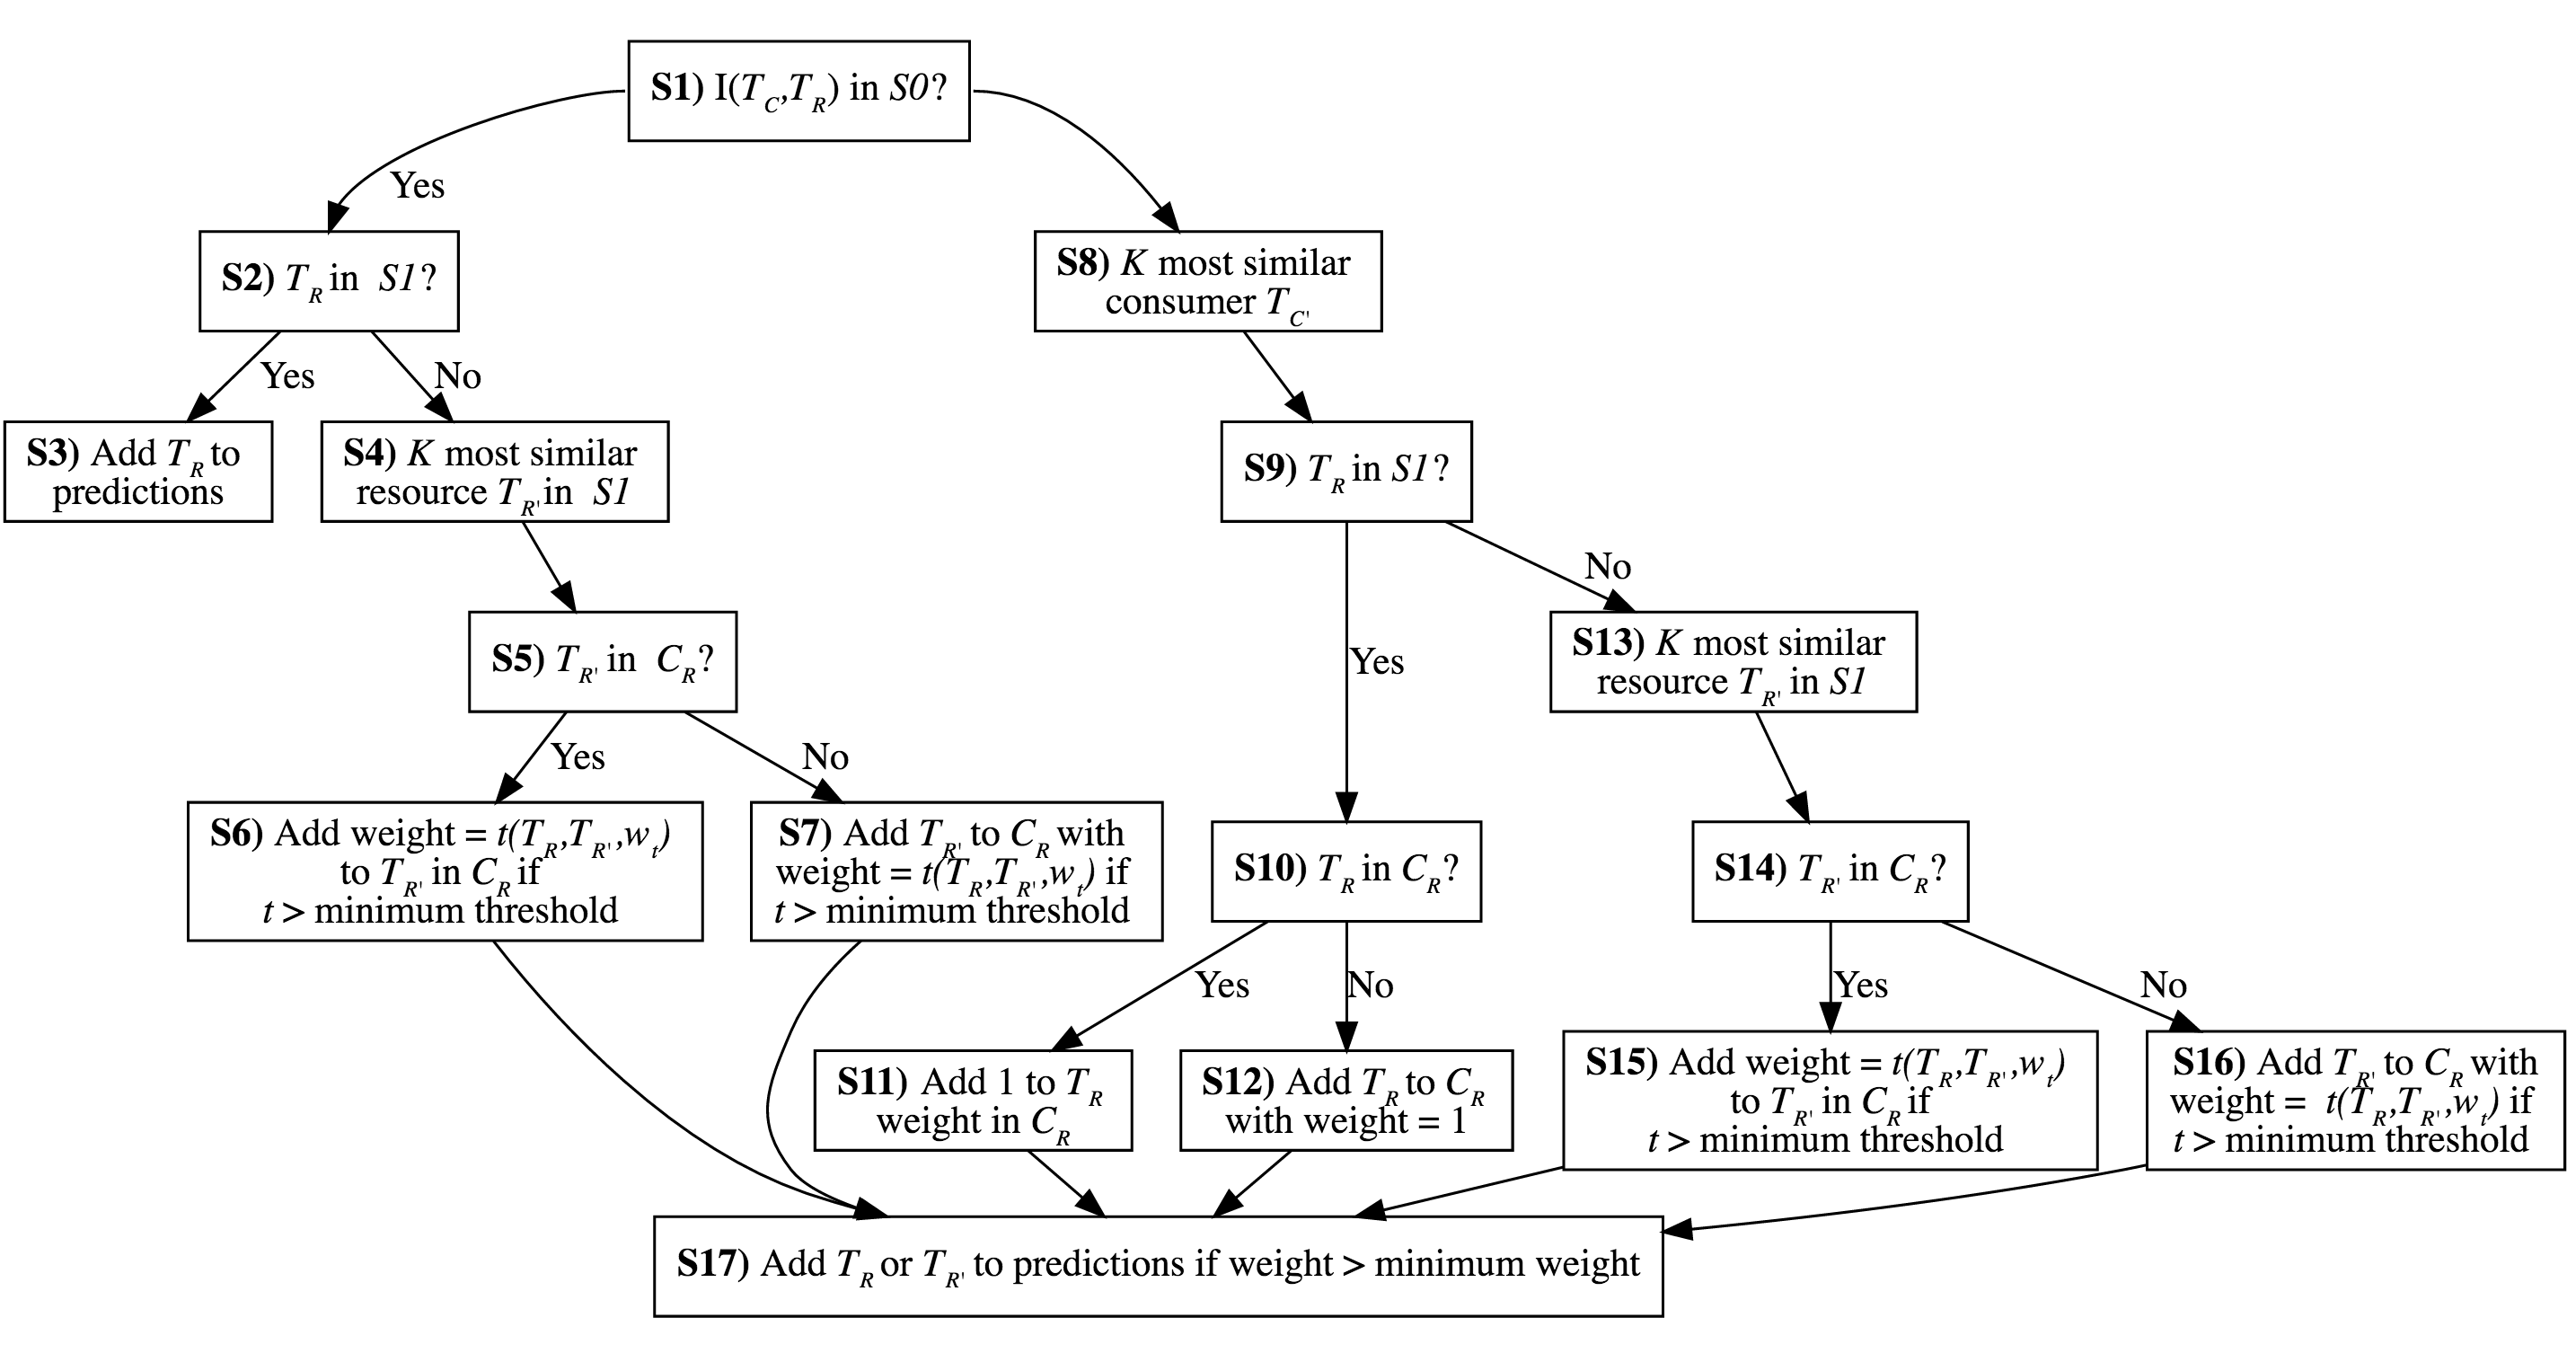
\includegraphics[width=0.85\textwidth]{Decision_Diagram.png}
      \caption{Description of the logical steps used by the algorithm to suggest a list of candidate resources ($C_R$) for each taxa ($T_C$) in \textit{S1}}
      \label{fig:decision_diag}
    \end{figure}

\newpage
    \begin{figure}[h]
      \centering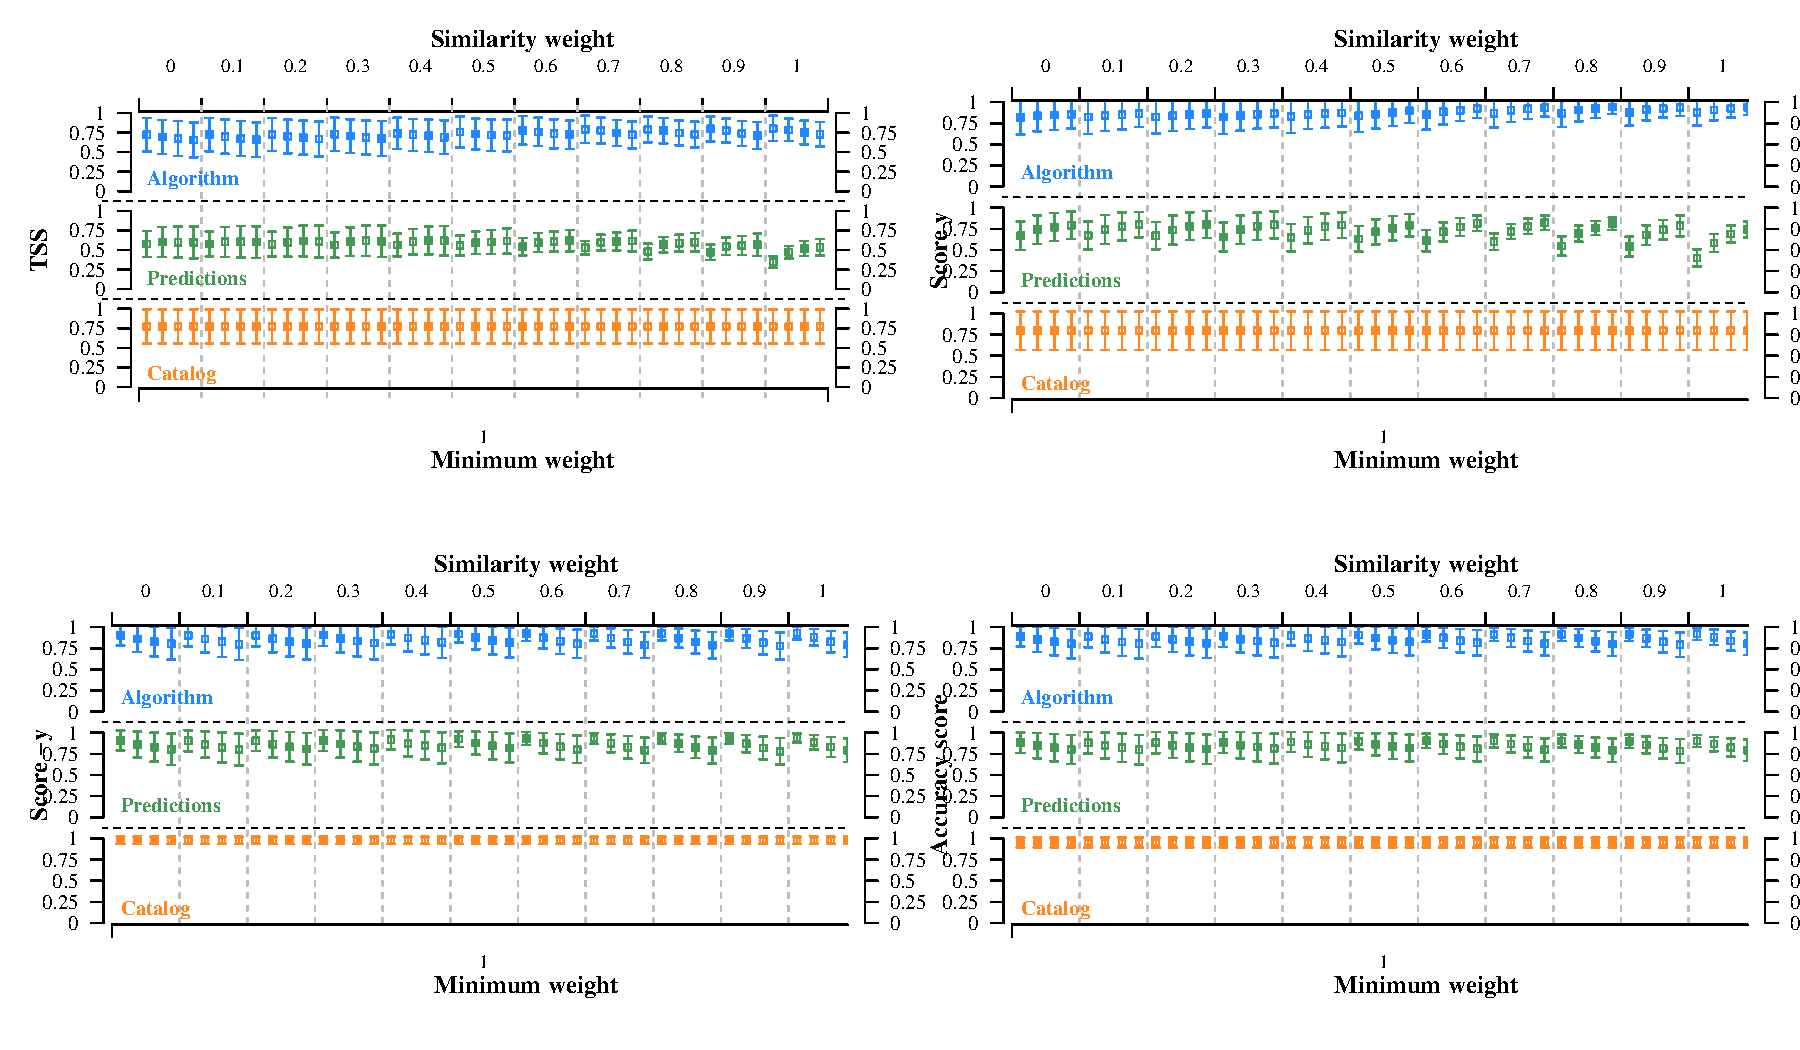
\includegraphics[width=0.85\textwidth, height=12cm]{multiple_parameters2.pdf}
      \caption{The graph presents the three statistics as a function of trait weight, which varies between 0 and 1. A weight of 0 means that similarity is measured only using set of resources for each taxa, while a weight equal to 1 means that similarity is based solely on taxonomy. We present 6 food webs with over 50 taxa each and the Barnes et al. (2008) dataset.}
      \label{fig:multi_param}
    \end{figure}

\newpage
    \begin{figure}[h]
      \centering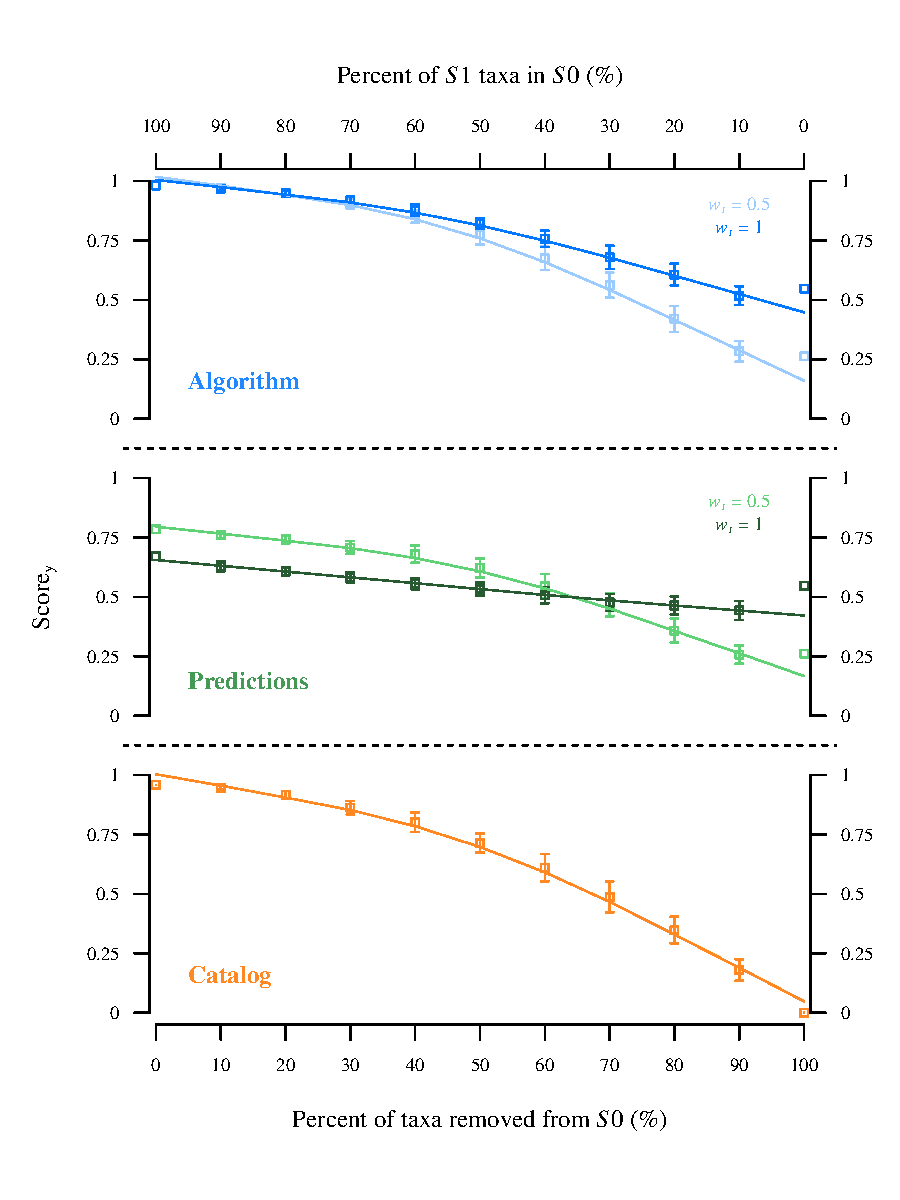
\includegraphics[width=0.85\textwidth]{catalog_predictions2.pdf}
      \caption{Graph presenting predictive accuracy as a function of the amount of information available in the catalogue. The arctic food web from Kortsch et al. (2015) was used for this, as it is highly detailed and because almost all taxa found in it had information in the catalogue even when not included in the catalogue. A random percentage of taxa in the web was iteratively removed from the catalogue (n = 50) before predicting interactions with the XXX algorithm.}
      \label{fig:catalog_pred}
    \end{figure}

\end{document}


% According to Eklof and Stouffer (2015), the phylogenetic component of food webs is a significant factor influencing the intervality of food webs. However, certain traits are not accounted by phylogenetic constraints, such as body size.

% predict* specie* interaction*
%
% Cite taxize
% Scott Chamberlain and Eduard Szocs (2013). taxize - taxonomic search and retrieval in R. F1000Research, 2:191. URL: http://f1000research.com/articles/2-191/v2.
%
% Scott Chamberlain, Eduard Szocs, Carl Boettiger, Karthik Ram, Ignasi Bartomeus, and John Baumgartner (2014) taxize: Taxonomic information from around the web. R package version 0.3.0.
% https://github.com/ropensci/taxize
%
% Jorrit H. Poelen, James D. Simons and Chris J. Mungall. (2014). Global Biotic Interactions: An open infrastructure to share and analyze species-interaction datasets. Ecological Informatics. http://dx.doi.org/10.1016/j.ecoinf.2014.08.005
%
% Bailly, N.; Boury-Esnault, N.; Brandão, S.N.; Costello, M.J.; Gofas, S.; Hernandez, F.; Horton, T.; Kroh, A.; Mees, J.; Paulay, G.; Poore, G.; Rosenberg, G.; Stöhr, S.; Decock, W.; Dekeyzer, S.; Vandepitte, L.; Vanhoorne, B.; Vranken, S.; Adams, M.J.; Adlard, R.; Adriaens, P.; Agatha, S.; Ahn, K.J.; Ahyong, S.; Alvarez, B.; Anderson, G.; Angel, M.; Arango, C.; Artois, T.; Atkinson, S.; Barber, A.; Bartsch, I.; Bellan-Santini, D.; Berta, A.; Bieler, R.; Błażewicz-Paszkowycz, M.; Bock, P.; Böttger-Schnack, R.; Bouchet, P.; Boyko, C.B.; Bray, R.; Bruce, N.L.; Cairns, S.; Campinas Bezerra, T.N.; Cárdenas, P.; Carstens, E.; Catalano, S.; Cedhagen, T.; Chan, B.K.; Chan, T.Y.; Cheng, L.; Churchill, M.; Coleman, C.O.; Collins, A.G.; Crandall, K.A.; Cribb, T.; Dahdouh-Guebas, F.; Daly, M.; Daneliya, M.; Dauvin, J.C.; Davie, P.; De Grave, S.; de Mazancourt, V.; Defaye, D.; d'Hondt, J.L.; Dijkstra, H.; Dohrmann, M.; Dolan, J.; Drapun, I.; Eisendle-Flöckner, U.; Eitel, M.; Encarnação, S.C.d.; Epler, J.; Ewers-Saucedo, C.; Faber, M.; Feist, S.; Finn, J.; Fišer, C.; Fonseca, G.; Fordyce, E.; Foster, W.; Frank, J.H.; Fransen, C.; Furuya, H.; Galea, H.; Garcia-Alvarez, O.; Gasca, R.; Gaviria-Melo, S.; Gerken, S.; Gheerardyn, H.; Gibson, D.; Gil, J.; Gittenberger, A.; Glasby, C.; Glover, A.; Gordon, D.; Grabowski, M.; Gravili, C.; Guerra-García, J.M..; Guidetti, R.; Guilini, K.; Guiry, M.D.; Hajdu, E.; Hallermann, J.; Hayward, B.; Hendrycks, E.; Herrera Bachiller, A.; Ho, J.s.; Høeg, J.; Holovachov, O.; Hooper, J.; Hughes, L.; Hummon, W.; Hyzny, M.; Iseto, T.; Ivanenko, S.; Iwataki, M.; Jarms, G.; Jaume, D..; Jazdzewski, K.; Kaminski, M.; Karanovic, I.; Kim, Y.H.; King, R.; Kirk, P.M.; Kolb, J.; Kotov, A.; Krapp-Schickel, T.; Kremenetskaia, A.; Kristensen, R.; Kullander, S.; La Perna, R.; Lambert, G.; Lazarus, D.; LeCroy, S.; Leduc, D.; Lefkowitz, E.J.; Lemaitre, R.; Lörz, A.N.; Lowry, J.; Macpherson, E.; Madin, L.; Mah, C.; Mamos, T.; Manconi, R.; Mapstone, G.; Marshall, B.; Marshall, D.J.; McInnes, S.; Meidla, T.; Meland, K.; Merrin, K.; Messing, C.; Miljutin, D.; Mills, C.; Mokievsky, V.; Molodtsova, T.; Monniot, F.; Mooi, R.; Morandini, A.C.; Moreira da Rocha, R.; Moretzsohn, F.; Mortelmans, J.; Mortimer, J.; Musco, L.; Neubauer, T.A.; Neuhaus, B.; Ng, P.; Nielsen, C.; Nishikawa, T.; Norenburg, J.; O'Hara, T.; Okahashi, H.; Opresko, D.; Osawa, M.; Ota, Y.; Parker, A.; Patterson, D.; Paxton, H.; Perrier, V.; Perrin, W.; Petrescu, I.; Picton, B.; Pilger, J.F.; Pisera, A.; Polhemus, D.; Pugh, P.; Reimer, J.D.; Reuscher, M.; Rius, M.; Rützler, K.; Rzhavsky, A.; Saiz-Salinas, J.; Santos, S.; Sartori, A.F.; Satoh, A.; Schatz, H.; Schierwater, B.; Schmidt-Rhaesa, A.; Schneider, S.; Schönberg, C.; Schuchert, P.; Self-Sullivan, C.; Senna, A.R.; Serejo, C.; Shamsi, S.; Sharma, J.; Shenkar, N.; Sicinski, J.; Siegel, V.; Sinniger, F.; Sivell, D.; Sket, B.; Smit, H.; Smol, N.; Souza-Filho, J.F..; Stampar, S.N.; Sterrer, W.; Stienen, E.; Strand, M.; Suárez-Morales, E.; Summers, M.; Suttle, C.; Swalla, B.J.; Taiti, S.; Tandberg, A.H.; Tang, D.; Tasker, M.; Taylor, J.; Tchesunov, A.; ten Hove, H.; ter Poorten, J.J.; Thomas, J.; Thuesen, E.V.; Thurston, M.; Thuy, B.; Timi, J.T.; Timm, T.; Todaro, A.; Turon, X.; Tyler, S.; Uetz, P.; Utevsky, S.; Vacelet, J.; Vader, W.; Väinölä, R.; van der Meij, S.E.; van Ofwegen, L.; van Soest, R.; Van Syoc, R.; Venekey, V.; Vonk, R.; Vos, C.; Walker-Smith, G.; Walter, T.C.; Watling, L.; Whipps, C.; White, K.; Williams, G.; Wilson, R.; Wyatt, N.; Wylezich, C.; Yasuhara, M.; Zanol, J.; Zeidler, W. (2016). World Register of Marine Species. Available from http://www.marinespecies.org at VLIZ. Accessed 2016-09-13. doi:10.14284/170






% \section{Figures et tableaux}
%
% \textit{Tables:}
% \begin{enumerate}
%   \item Description of empirical data used to obtain list of binary interactions
%   \item Description of empirical binary interactions and data availability for large taxonomic groups (e.g. mammals, fish, benthic invertebrates). Needs to be defined.
% \end{enumerate}
%
% \textit{Figures:}
% \begin{enumerate}
%   \item Predicting empirical food webs from empirical data catalogue. Figure of results \% efficiency as a function of the number of taxa in the food web. All species-species interactions of each empirical food web removed from empirical biotic interaction catalogue.
%   \item Predicting interactions with differing levels of taxonomic resolution. (e.g. interactions aggregated at the species, genus, family level)
%   \item Efficiency of predictions for large taxonomic groups.
%   \item Representing the St. Lawrence food web. Heatmap with phylogeny as axes. Package heatmap3.
% \end{enumerate}
%
% \textit{Figure additionnelle mais peut-être pas pour cet article?:}
% \begin{enumerate}
%   \item Predictive accuracy of method as a function of the amount of data available in the catalogue for large taxonomic groups. The idea would be to discuss the amount of data required in ``biological compartments'' for the learning method to be efficient.
% \end{enumerate}

% We selected a list of species forming the known biodiversity of the estuary and gulf of St. Lawrence in Canada. The species list available on CaRMS (ref) for this region was selected, and completed with a comprehensive list of marine birds (Allard et al. 2013) and marine mammals (Lesage, personnal communication), for a total of 1469 species.
% The data compilation process yielded a total of 276708 binary interactions (interactions = 72110; non-interactions = 204598) for 9712 taxa (Superfamily = 15; Family = 591; Subfamily = 29; Tribe = 8; Genus = 1972; Species = 7097). Of that number, interactions for St. Lawrence taxa were described for 33\% of species, 64\% of genera and 82\% of families, although these interactions are not necessarily between two taxa found in the St. Lawrence.
